\documentclass{standalone}
\usepackage{tikz}
\usetikzlibrary{patterns, positioning}
\usepackage[sfdefault]{ClearSans} %% option 'sfdefault' activates Clear Sans as the default text font
\usepackage[T1]{fontenc}

\begin{document}
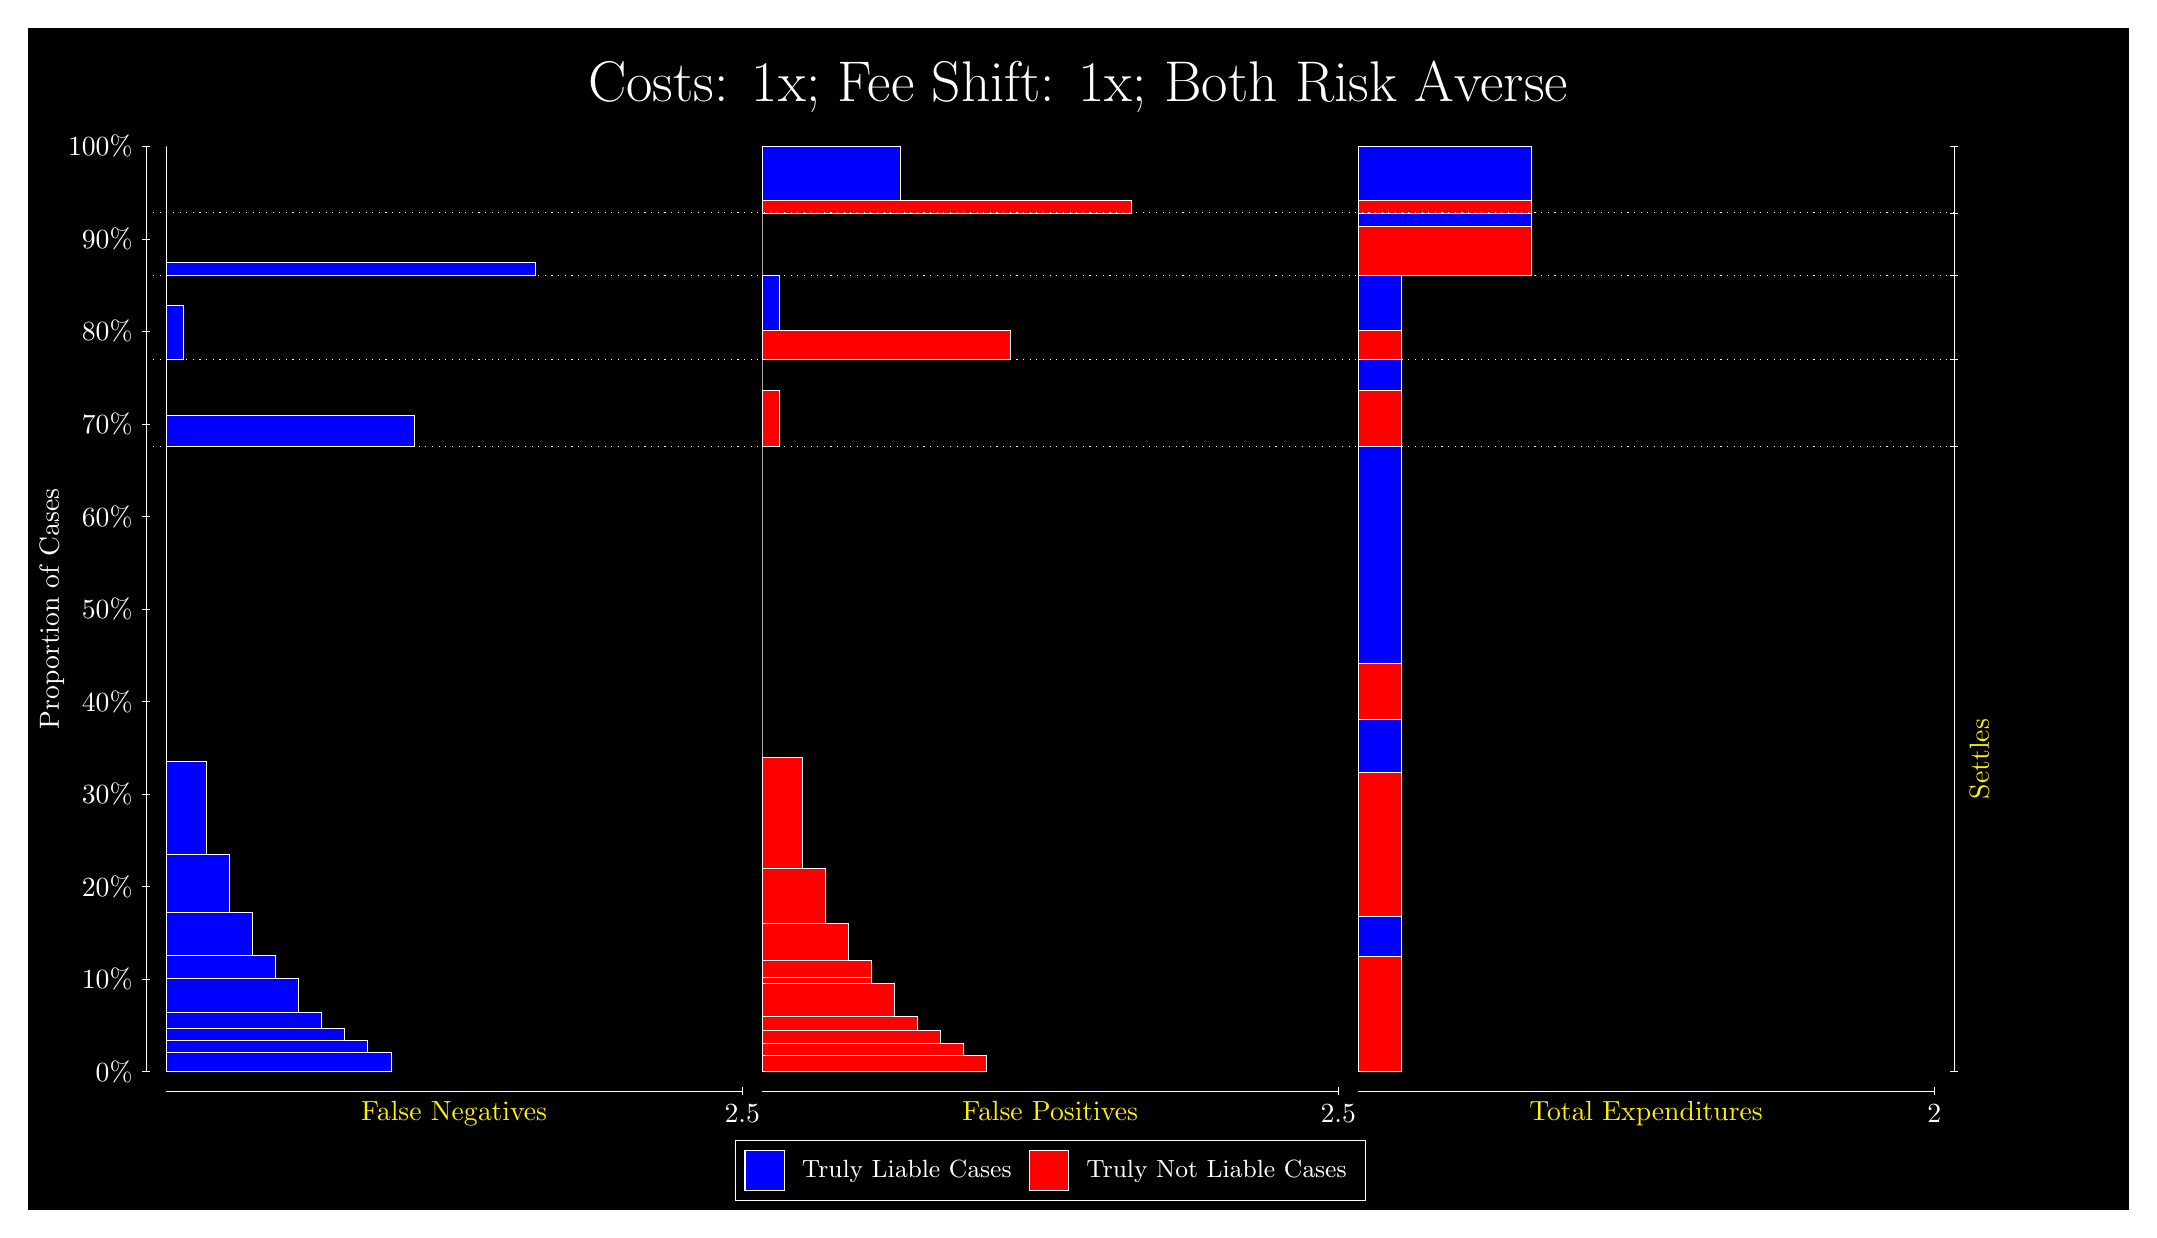
\begin{tikzpicture}
\draw[fill=black] (0,0) rectangle (26.667,15);
\draw[text=white] (0,13.5) rectangle (26.667,15) node[midway] {\huge Costs: 1x; Fee Shift: 1x; Both Risk Averse};
\draw[white, very thin] (1.5,1.75) -- (1.5,13.5);
\node[rotate=90, text=white, anchor=center] at (0.3, 7.625) {Proportion of Cases};
\draw[white, very thin] (1.45,1.75) -- (1.55,1.75);
\node[text=white, anchor=east] at (1.45, 1.75) {0\%};
\draw[white, very thin] (1.45,2.925) -- (1.55,2.925);
\node[text=white, anchor=east] at (1.45, 2.925) {10\%};
\draw[white, very thin] (1.45,4.1) -- (1.55,4.1);
\node[text=white, anchor=east] at (1.45, 4.1) {20\%};
\draw[white, very thin] (1.45,5.275) -- (1.55,5.275);
\node[text=white, anchor=east] at (1.45, 5.275) {30\%};
\draw[white, very thin] (1.45,6.45) -- (1.55,6.45);
\node[text=white, anchor=east] at (1.45, 6.45) {40\%};
\draw[white, very thin] (1.45,7.625) -- (1.55,7.625);
\node[text=white, anchor=east] at (1.45, 7.625) {50\%};
\draw[white, very thin] (1.45,8.8) -- (1.55,8.8);
\node[text=white, anchor=east] at (1.45, 8.8) {60\%};
\draw[white, very thin] (1.45,9.975) -- (1.55,9.975);
\node[text=white, anchor=east] at (1.45, 9.975) {70\%};
\draw[white, very thin] (1.45,11.15) -- (1.55,11.15);
\node[text=white, anchor=east] at (1.45, 11.15) {80\%};
\draw[white, very thin] (1.45,12.325) -- (1.55,12.325);
\node[text=white, anchor=east] at (1.45, 12.325) {90\%};
\draw[white, very thin] (1.45,13.5) -- (1.55,13.5);
\node[text=white, anchor=east] at (1.45, 13.5) {100\%};

\draw[white, very thin] (24.457,1.75) -- (24.457,13.5);
\draw[white, very thin] (24.407,1.75) -- (24.507,1.75);
\node[anchor=west] at (24.407, 1.75) {};
\draw[white, very thin] (24.407,9.688) -- (24.507,9.688);
\node[anchor=west] at (24.407, 9.688) {};
\draw[white, very thin] (24.407,10.794) -- (24.507,10.794);
\node[anchor=west] at (24.407, 10.794) {};
\draw[white, very thin] (24.407,11.859) -- (24.507,11.859);
\node[anchor=west] at (24.407, 11.859) {};
\draw[white, very thin] (24.407,12.654) -- (24.507,12.654);
\node[anchor=west] at (24.407, 12.654) {};
\draw[white, very thin] (24.407,13.5) -- (24.507,13.5);
\node[anchor=west] at (24.407, 13.5) {};

\draw[white, very thin, fill=blue] (1.75,1.75) rectangle (4.6044,1.9929);
\draw[white, very thin, fill=blue] (1.75,1.9929) rectangle (4.3116,2.149);
\draw[white, very thin, fill=blue] (1.75,2.149) rectangle (4.0188,2.2937);
\draw[white, very thin, fill=blue] (1.75,2.2937) rectangle (3.7261,2.5031);
\draw[white, very thin, fill=blue] (1.75,2.5031) rectangle (3.4333,2.9361);
\draw[white, very thin, fill=blue] (1.75,2.9361) rectangle (3.1406,3.2209);
\draw[white, very thin, fill=blue] (1.75,3.2209) rectangle (2.8478,3.7776);
\draw[white, very thin, fill=blue] (1.75,3.7776) rectangle (2.5551,4.5085);
\draw[white, very thin, fill=blue] (1.75,4.5085) rectangle (2.2623,5.6945);
\draw[white, very thin, fill=red] (1.75,5.6945) rectangle (1.75,9.688);
\draw[white, very thin, fill=blue] (1.75,9.688) rectangle (4.8971,10.081);
\draw[white, very thin, fill=red] (1.75,10.081) rectangle (1.75,10.794);
\draw[white, very thin, fill=blue] (1.75,10.794) rectangle (1.9696,11.485);
\draw[white, very thin, fill=red] (1.75,11.485) rectangle (1.75,11.859);
\draw[white, very thin, fill=blue] (1.75,11.859) rectangle (6.4341,12.023);
\draw[white, very thin, fill=red] (1.75,12.023) rectangle (1.75,12.654);
\draw[white, very thin, fill=red] (1.75,12.654) rectangle (1.75,12.818);
\draw[white, very thin, fill=blue] (1.75,12.818) rectangle (1.75,13.5);
\draw[white, very thin, fill=red] (9.3189,1.75) rectangle (12.173,1.9574);
\draw[white, very thin, fill=red] (9.3189,1.9574) rectangle (11.88,2.1109);
\draw[white, very thin, fill=red] (9.3189,2.1109) rectangle (11.588,2.2699);
\draw[white, very thin, fill=red] (9.3189,2.2699) rectangle (11.295,2.4516);
\draw[white, very thin, fill=red] (9.3189,2.4516) rectangle (11.002,2.877);
\draw[white, very thin, fill=red] (9.3189,2.877) rectangle (10.709,2.9484);
\draw[white, very thin, fill=red] (9.3189,2.9484) rectangle (10.709,3.1677);
\draw[white, very thin, fill=red] (9.3189,3.1677) rectangle (10.417,3.6279);
\draw[white, very thin, fill=red] (9.3189,3.6279) rectangle (10.124,4.3371);
\draw[white, very thin, fill=red] (9.3189,4.3371) rectangle (9.8312,5.7434);
\draw[white, very thin, fill=blue] (9.3189,5.7434) rectangle (9.3189,9.688);
\draw[white, very thin, fill=red] (9.3189,9.688) rectangle (9.5384,10.401);
\draw[white, very thin, fill=blue] (9.3189,10.401) rectangle (9.3189,10.794);
\draw[white, very thin, fill=red] (9.3189,10.794) rectangle (12.466,11.168);
\draw[white, very thin, fill=blue] (9.3189,11.168) rectangle (9.5384,11.859);
\draw[white, very thin, fill=red] (9.3189,11.859) rectangle (9.3189,12.489);
\draw[white, very thin, fill=blue] (9.3189,12.489) rectangle (9.3189,12.654);
\draw[white, very thin, fill=red] (9.3189,12.654) rectangle (14.003,12.818);
\draw[white, very thin, fill=blue] (9.3189,12.818) rectangle (11.075,13.5);
\draw[white, very thin, fill=red] (16.888,1.75) rectangle (17.437,3.2102);
\draw[white, very thin, fill=blue] (16.888,3.2102) rectangle (17.437,3.7204);
\draw[white, very thin, fill=red] (16.888,3.7204) rectangle (17.437,5.5521);
\draw[white, very thin, fill=blue] (16.888,5.5521) rectangle (17.437,6.2279);
\draw[white, very thin, fill=red] (16.888,6.2279) rectangle (17.437,6.9295);
\draw[white, very thin, fill=blue] (16.888,6.9295) rectangle (17.437,9.688);
\draw[white, very thin, fill=red] (16.888,9.688) rectangle (17.437,10.401);
\draw[white, very thin, fill=blue] (16.888,10.401) rectangle (17.437,10.794);
\draw[white, very thin, fill=red] (16.888,10.794) rectangle (17.437,11.168);
\draw[white, very thin, fill=blue] (16.888,11.168) rectangle (17.437,11.859);
\draw[white, very thin, fill=red] (16.888,11.859) rectangle (19.083,12.489);
\draw[white, very thin, fill=blue] (16.888,12.489) rectangle (19.083,12.654);
\draw[white, very thin, fill=red] (16.888,12.654) rectangle (19.083,12.818);
\draw[white, very thin, fill=blue] (16.888,12.818) rectangle (19.083,13.5);
\draw[white, dotted] (1.5,9.688) -- (24.457,9.688);
\draw[white, dotted] (1.5,10.794) -- (24.457,10.794);
\draw[white, dotted] (1.5,11.859) -- (24.457,11.859);
\draw[white, dotted] (1.5,12.654) -- (24.457,12.654);
\draw[white, very thin] (1.75,1.5) -- (9.0689,1.5);
\node[text=yellow, anchor=north] at (5.4094, 1.5) {False Negatives};
\draw[white, very thin] (9.0689,1.45) -- (9.0689,1.55);
\node[text=white, anchor=north] at (9.0689, 1.45) {2.5};

\draw[white, very thin] (9.3189,1.5) -- (16.638,1.5);
\node[text=yellow, anchor=north] at (12.978, 1.5) {False Positives};
\draw[white, very thin] (16.638,1.45) -- (16.638,1.55);
\node[text=white, anchor=north] at (16.638, 1.45) {2.5};

\draw[white, very thin] (16.888,1.5) -- (24.207,1.5);
\node[text=yellow, anchor=north] at (20.547, 1.5) {Total Expenditures};
\draw[white, very thin] (24.207,1.45) -- (24.207,1.55);
\node[text=white, anchor=north] at (24.207, 1.45) {2};

\node[text=yellow, centered, rotate=90] at (24.777, 5.719) {Settles};





\draw (12.978300999999998,1.5) node[draw=none] (baseCoordinate) {};
\begin{scope}[align=center]
        \matrix[scale=0.5, draw=white, below=0.5cm of baseCoordinate, nodes={draw}, column sep=0.1cm]{
            \node[rectangle, draw, minimum width=0.5cm, minimum height=0.5cm, fill=blue] {}; &
            \node[draw=none, font=\small, text=white] (B) {Truly Liable Cases}; &
            \node[rectangle, draw, minimum width=0.5cm, minimum height=0.5cm, fill=red] {}; &
            \node[draw=none, font=\small, text=white] (B) {Truly Not Liable Cases}; \\
            };
\end{scope}

\end{tikzpicture}
\end{document}